% 3장 채널 부호화 (원문 pp. 20--31, 식 (17)--(33), 그림 4--5)
\section{채널 부호화}

채널 부호화의 기본 과제는 잡음이 있는 채널로 $M$개의 메시지를 보내되, 수신단에서 이들을 신뢰성 있게 구별할 수 있게 하는 것이다. 이 장에서는 채널 부호화의 정보이론적 근본 한계에 관한 최근 진전을 살펴본다. 특히 P2P 채널, 다중 접속 채널, 대규모 접속 채널에 초점을 둔다.

\subsection{P2P 채널}

\subsubsection{핵심 지표}

Shannon이 세운 통신의 기본 틀 [8]은 채널 부호화를 다음 네 가지 핵심 구성 요소로 정식화한다.
1) 사전에 알려지지 않은 메시지. 이 메시지는 집합 $\{1,\dots,M\}$ 위에서 균등한 확률변수 $W$로 모형화한다.
2) 부호기 $\ff:\{1,\dots,M\}\to\mathcal{X}^n$. 부호기는 메시지 $W$를 길이 $n$인 부호어 $X^n$으로 사상한다.
3) 채널. 채널은 입력 $x^n\in\mathcal{X}^n$과 출력 $y^n\in\mathcal{Y}^n$을 잇는 무작위 변환의 수열 $P_{Y^n|X^n}$으로 모형화한다.
4) 복호기 $\gg:\mathcal{Y}^n\to\{1,\dots,M\}$. 복호기는 채널 출력 $Y^n$을 바탕으로 메시지의 추정값 $\widehat{W}$를 내놓는다.

$(n,M,\epsilon)$-부호란 부호 길이가 $n$이고 부호책 크기가 $M$이며, 복호 오류 확률이 $\epsilon$ 이하임을 보장하는 부호기-복호기 쌍 $(\ff,\gg)$를 말한다. 흔히 쓰는 오류 제약은 두 가지로, 평균 오류 확률 제약과 최대 오류 확률 제약이다. 각각 다음과 같다.
\begin{align}
P_{\mathrm{e,ave}} &= \P\bigl[\widehat{W}\neq W\bigr]\le\epsilon, \tag{17}\\
P_{\mathrm{e,max}} &= \max_{1\le j\le M}\P\bigl[\widehat{W}\neq W \,\big|\, W=j\bigr]\le\epsilon. \tag{18}
\end{align}
율(rate)은 $R\triangleq\frac{\log M}{n}$으로 정의하며, 단위는 채널 사용당 비트이다. 부호 길이 $n$과 목표 오류 확률 $\epsilon$이 주어졌을 때의 최대 데이터율을 나타내는 근본 한계 $R^\star(n,\epsilon)$은 다음과 같이 정의한다.
\begin{equation}
R^\star(n,\epsilon)\triangleq\sup\left\{R:\exists\,(n,M,\epsilon)-\text{code}\right\}. \tag{19}
\end{equation}
마찬가지로, 달성할 수 있는 가장 작은 오류 확률은 다음과 같이 정의한다.
\begin{equation}
\epsilon^\star(n,R)\triangleq\sup\left\{\epsilon:\exists\,(n,2^{nR},\epsilon)-\text{code}\right\}. \tag{20}
\end{equation}
\onote{본문은 ``가장 작은'' 오류 확률이라고 하므로, 식 (20)의 $\sup$은 $\inf$여야 맞다. 여기서는 원문대로 옮겼다.}

\subsubsection{고전적 점근 결과}

Shannon의 선구적 연구 [8]는 $(n,\epsilon)$ 쌍이 주어졌을 때 $R^\star(n,\epsilon)$을 분석하는 이론적 토대를 놓았다. Shannon이 관찰한 놀라운 사실은, 부호 길이 $n$이 무한대로 가고 오류 확률 $\epsilon$이 0으로 가면 $R^\star(n,\epsilon)$을 점근적으로 다룰 수 있게 된다는 것이다. 이때 $R^\star(n,\epsilon)$의 점근 극한을 채널 용량 $C$라 한다. 즉,
\begin{equation}
C=\lim_{\epsilon\to0}\lim_{n\to\infty}R^\star(n,\epsilon). \tag{21}
\end{equation}
이 식은 부호 길이가 충분히 길기만 하면 용량보다 낮은 어떤 율에서도 오류 없는 전송이 가능함을 보여 준다. 무기억 채널 $P_{Y|X}$의 채널 용량 $C$는 다음과 같이 쓸 수 있다 [8], [66, Sec.~7].
\begin{equation}
C=\sup_{P_X}I(X;Y), \tag{22}
\end{equation}
여기서 $I(X;Y)$는 $X$와 $Y$ 사이의 단일 문자 상호 정보량이고, 상한은 모든 입력 분포에 대해 취한다. $\epsilon>0$을 고정하고 $n\to\infty$로 보낼 때 $R^\star(n,\epsilon)$의 극한을 $\epsilon$-용량 $C_\epsilon$이라 한다. 즉,
\begin{equation}
C_\epsilon=\lim_{n\to\infty}R^\star(n,\epsilon). \tag{23}
\end{equation}

율 $R$을 고정하면, $\epsilon^\star(n,R)$의 점근적 거동은 신뢰도 함수 $E(R)$이 결정한다. 즉,
\begin{equation}
E(R)=\liminf_{n\to\infty}-\frac{\log\epsilon^\star(n,R)}{n}. \tag{24}
\end{equation}
율 $R$이 용량 $C$를 넘으면 통신은 신뢰할 수 없고, 이때 $E(R)=0$이다. 반면 $R<C$로 제한하면 오류 확률은 지수 $E(R)>0$으로 지수적으로 감소할 수 있다.

\subsubsection{비점근 한계}

고전 정보이론은 무한한 부호 길이, 무한한 페이로드 크기, 사라지는 오류 확률 가운데 일부 또는 전부를 가정한다. 그래서 짧은 부호 길이와 짧은 패킷을 쓰고, 작지만 무시할 수 없는 오류 확률을 요구하는 실제 통신 시스템의 근본 한계는 규명하지 못한다. 이 문제를 피하고자 여러 연구가 유한 부호 길이 정보이론에 집중해 왔다. 유한 부호 길이 영역에서는 단순한 이진 대칭 채널이나 이진 소거 채널에서조차 최대 율 $R^\star(n,\epsilon)$을 정확히 계산하기가 계산상 불가능하다. 이 때문에 연구자들은 달성 가능성 쪽과 역 쪽 모두에서 촘촘하면서도 계산 가능한 한계를 개발하게 되었다. 아래에서는 몇 가지 비점근 한계와 그 유도에 쓰인 핵심 아이디어를 살펴본다.

\paragraph{1) 달성 가능성 한계}
Feinstein [94]과 Shannon [95]은 각각 최대 부호화와 무작위 부호화 아이디어에 기초하여 $R^\star(n,\epsilon)$에 대한 유한 부호 길이 달성 가능성 한계(곧 하한)를 세웠다. 무작위 부호화 아이디어에서는 어떤 분포로부터 부호책을 무작위로 구성한 뒤, 앙상블의 여러 실현에 걸쳐 오류 확률을 평가한다. 이로써 평균 오류 확률 제약 아래에서 부호가 존재함을 증명한다. 최대 부호화 방식에서는 최대 오류 확률 제약을 어기게 될 때까지 부호어를 하나씩 차례로 덧붙인다. 문헌에 있는 달성 가능성 한계는 거의 모두 이 두 아이디어를 바탕으로 한다. 한계 사이의 차이는 주로 복호 규칙(전형성 복호, 최대 우도 복호, 문턱값 복호 등)과 오류 분석 기법에 있다. 예를 들어 Polyanskiy, Poor, Verdú [11]는 $R^\star(n,\epsilon)$에 대해 해석적으로 다루기 쉽고 비점근적으로도 날카로운 달성 가능성 한계를 여럿 유도했는데, 의존성 검정(DT, dependence-testing) 한계와 $\kappa\beta$ 한계가 그 예이다. 이러한 달성 가능성 한계를 유도하는 핵심 원리는 무작위/최대 부호화와 가설 검정이다. $R^\star(n,\epsilon)$에 대한 한계와 별도로, Gallager [96]는 신뢰도 함수 분석에 더 알맞은 달성 가능성 한계를 유도했다(최근 개관은 [97] 참고). 또한 [32]에서는 점근적 황금 공식(golden formula)과 비점근 $\beta\beta$ 한계 사이의 관계를 규명했다. 도청 채널의 비점근 근본 한계는 [98]에서 탐구했다.

위의 한계는 전력 제약이 있는 시스템으로 자연스럽게 일반화할 수 있다. 입력 분포는 유한 부호 길이 성능을 크게 좌우한다. 대부분의 부호어 전력을 쓸 수 있는 최대 전력 예산 근처에 모으면 성능이 크게 좋아진다. 그래서 [11]과 [99]는 1차 최적인 i.i.d.\ 가우스 부호어 대신 전력 껍질에서 뽑은 부호어의 입력 앙상블을 썼다. Gallager는 얇은 껍질 안에 놓인 절단 가우스 분포로 부호어를 생성하는 방법을 제안했다 [100]. 아울러 위의 결과는 되먹임이 있는 채널로도 일반화할 수 있다. 구체적으로, Polyanskiy 등 [33]은 오류 확률이 고정되고 평균 복호 시간이 유한할 때 달성할 수 있는 최대 부호책 크기에 대한 비점근 한계를 유도했고, 이 한계는 [34]에서 더 개선되었다. [34]의 저자들은 또한 평균 전력 제약이 있는 이산 무기억 채널과 AWGN 채널(가산 백색 가우스 잡음 채널)에 대해, 바탕에 있는 채널 매개변수를 몰라도 되는 범용 가변 길이 되먹임 부호를 개발했다.

\paragraph{2) 역 한계}
문헌에는 역 한계가 많이 세워져 있다. Fano 부등식은 $R^\star(n,\epsilon)$에 대한 약한 역 한계(곧 상한)를 증명하는 고전적 도구이다 [66, Sec.~7.9]. 한편 Wolfowitz [101]는 이산 무기억 채널에 대한 강한 역 한계를 세웠다. [102]의 저자들은 신뢰도 함수 분석에 알맞은 구 채우기 역 한계를 유도했다. Verdú와 Han [103]은 정보 스펙트럼(information spectrum)에 기초한 역 한계를 세웠는데, 이 한계는 임의의 무작위 변환에 대해 성립한다. 이후 Polyanskiy, Poor, Verdú는 가설 검정과 여러 데이터 처리 부등식에 기초하여 메타 역정리 한계라는 일반적인 역 한계를 유도했다 [65]. [65, Sec.~2.7.3]과 [35]에서는 대부분의 역 결과를 이 메타 역정리 한계로부터 되찾을 수 있음을 보였다.

\paragraph{3) 수치 결과}
그림~4는 P2P AWGN 채널에서 최대 전력 제약 아래 $R^\star(n,\epsilon)$에 대한 여러 달성 가능성 한계와 역 한계를 비교한다. 비점근 한계와 점근 용량 사이의 간격이 크다는 점에서, $n$과 $\log M$이 작은 짧은 패킷 통신에 유한 부호 길이 정보이론을 적용하는 일이 얼마나 중요한지 드러난다. 비점근 달성 가능성 한계 가운데 Shannon 한계가 가장 촘촘하지만, AWGN에 특화된 설정에만 쓸 수 있다. $\kappa\beta$ 한계는 Shannon 한계보다 조금 느슨하지만, 점근 분석에서 계산상 더 다루기 쉽고 더 일반적이다. Feinstein 한계는 $\kappa\beta$ 한계보다 느슨하다. $\kappa\beta$ 한계는 Gallager 한계와 비교하면 $n$이 큰 영역에서는 더 촘촘하지만 $n$이 작을 때는 더 느슨하다. 그림~4에는 저복잡도 신뢰 전파(belief propagation) 기반 복호기를 쓰는 다중 에지(multi-edge) 저밀도 패리티 검사(LDPC, low-density parity-check) 부호의 성능도 함께 나와 있다. 이 실용 기법을 용량과 비교하면, $n$이 커질수록 기법이 최적에 가까워짐을 알 수 있다. 그러나 이 기법과 유한 부호 길이 한계 사이의 간격은 부호 길이와 거의 무관하다. 이 불일치는 부호 설계를 평가하는 패러다임이 바뀌어야 함을 보여 준다. 즉 짧은 패킷 통신의 성능을 정확히 평가하려면 점근 지표를 넘어 유한 부호 길이 정보이론을 받아들여야 한다.

차세대 채널 부호화는 6G의 엄격한 요구 사항을 만족해야 할 뿐 아니라, 이미 빽빽한 기저대역 칩에 부담을 더 얹지 않도록 하위 호환성도 갖추어야 한다. 이런 배경에서 [104]의 저자들은 6G 통신을 위한 후보 채널 부호를 검토하고, LDPC와 폴라(polar) 틀에 기초한 차세대 채널 부호를 탐구했다. [104]에서는 폴라 유사 성분을 지닌 일반화 LDPC(GLDPC-PC, generalized LDPC with polar-like component) 부호라는 새로운 개념을 도입했다. 이 부호에서는 폴라 성분이 변수 노드로 넘기는 연판정 정보(soft information)를 연출력 연속 제거 목록(SO-SCL, soft-output successive cancellation list) 복호기 [105]로부터 효율적으로 추출한다. 그런데 연속 제거 목록 복호는 본질적으로 순차적이어서 SO-SCL 복호기의 복호 지연이 크다. 이를 고려하여 [106]의 저자들은 노드 기반 고속 복호를 SO-SCL 틀에 결합한 연출력 고속 SCL(SO-FSCL) 복호기를 제안했다. 더 자세한 내용은 [104, 105, 106]을 참고하라.

\begin{figure}[t]
\centering
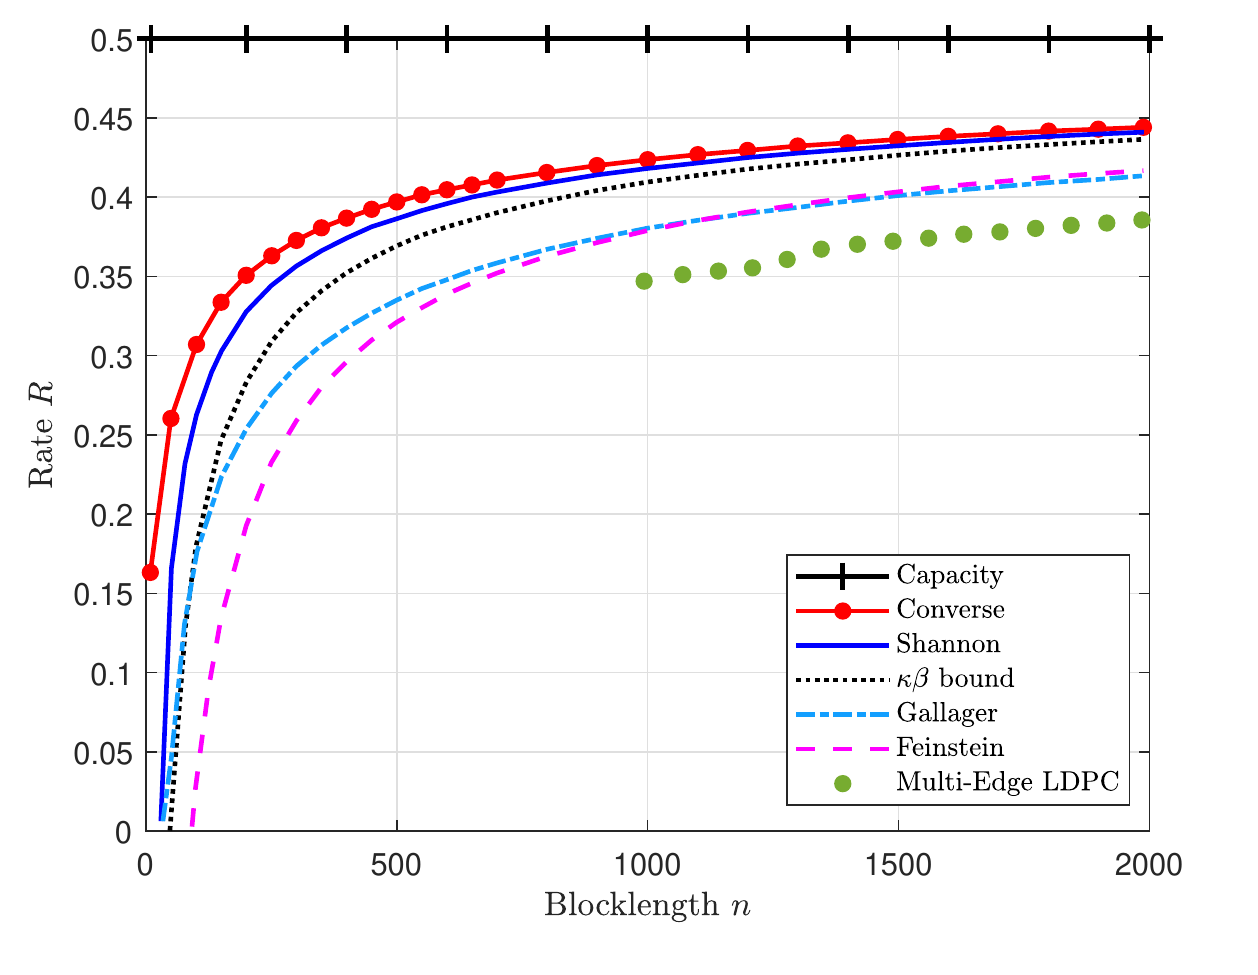
\includegraphics[width=0.85\linewidth]{fig/fig4.png}
\caption{SNR $=0$\,dB, $\epsilon=10^{-3}$인 AWGN 채널에서 P2P 통신의 이론적 한계와 다중 에지 LDPC 알고리즘.}
\end{figure}

\subsubsection{근사}

무선 통신 시스템 설계에 공학적 통찰을 주려면, 상한과 하한보다 계산 복잡도가 낮으면서 다루기 쉬운 $R^\star(n,\epsilon)$의 근사를 개발하는 일이 매우 중요하다. 이를 위한 분석 기법으로는 서로 보완적인 세 가지, 곧 CLT, 대편차(LD), 중편차(MD, moderate deviations)가 있으며, 아래에서 차례로 소개한다.

Polyanskiy, Poor, Verdú [11]는 Strassen [73]의 고전적 전개 결과를 바탕으로, CLT 영역에서는 채널의 2차 통계량인 채널 분산도를 도입하면 최대 부호율 $R^\star(n,\epsilon)$을 촘촘하게 근사할 수 있음을 보였다. 채널 분산도는 다음과 같이 정의한다 [11, Def.~1].
\begin{equation}
V=\lim_{\epsilon\to0}\lim_{n\to\infty}n\left(\frac{C-R^\star(n,\epsilon)}{Q^{-1}(\epsilon)}\right)^{2}. \tag{25}
\end{equation}
용량 $C$가 양수인 여러 채널에서 최대 부호율 $R^\star(n,\epsilon)$은 정규 근사 [11]로 촘촘하게 근사된다.
\begin{equation}
R^\star(n,\epsilon)=C-\sqrt{\frac{V}{n}}\,Q^{-1}(\epsilon)+O\!\left(\frac{\log n}{n}\right). \tag{26}
\end{equation}
이 근사에 따르면, 부호 길이 $n$에서 오류 확률을 $\epsilon$ 이하로 보장하려면 율 면에서 (채널 용량에 비해) $\frac{1}{\sqrt{n}}$에 비례하는 손실을 치러야 한다. 부호 길이 $n$이 무한대로 가면 이 율 손실은 0으로 간다.

신호 대 잡음비(SNR, signal-to-noise ratio)가 $P$인 AWGN 채널에서 $C$와 $V$는 다음과 같다 [11, Theorem~54].
\begin{align}
C &= \frac{1}{2}\log(1+P), \tag{27}\\
V &= \frac{P}{2}\,\frac{(2+P)}{(1+P)^2}\log^2 e. \tag{28}
\end{align}
[11]의 결과는 여러 무선 통신 채널로 일반화되었다. 페이딩 계수가 한 부호어 동안 변하지 않는 MIMO 준정적 페이딩 채널에서는, [36, Theorem~3]에 제시된 페이딩 분포에 대한 완만한 조건 아래 채널 분산도가 0임이 증명되었다. 즉 다음이 성립한다 [36].
\begin{equation}
R^\star(n,\epsilon)=C_\epsilon+O\!\left(\frac{\log n}{n}\right). \tag{29}
\end{equation}
채널 분산도는 에르고딕 페이딩 채널에 대해서도 연구되었다. 구체적으로, 수신단에 채널 상태 정보(CSI, channel state information)가 알려진 단일 입력 단일 출력(SISO, single-input single-output) 정상 페이딩 채널의 분산도는 [37]에서 유도되었다. 이 결과는 [107]에서 SISO 블록 무기억 페이딩 채널로, [38]에서 다중 입력 다중 출력(MIMO, multiple-input multiple-output) 블록 무기억 페이딩 채널로 확장되었다. 안테나 수가 부호 길이에 비례하여 늘어나는 점근적 에르고딕 설정에 대해서는, [39]가 MIMO 준정적 레일리(Rayleigh) 페이딩 채널의 2차 부호율에 대한 상한과 하한을 제시했다. You 등 [40]은 대규모 MIMO 시스템에서 달성 가능한 율의 상한에 대한 닫힌 형태의 근사를 다음과 같이 유도했다.
\begin{equation}
\frac{R^\star(n,\epsilon)}{m}\le\log(1+P)-\sqrt{\frac{1}{nm}}\,Q^{-1}(\epsilon), \tag{30}
\end{equation}
여기서 $m$은 공간 자유도이다. 이 식에서 $mn$ 값을 고정하면 Hz당·안테나당 평균 데이터율이 변하지 않음을 알 수 있다. 이는 $n$과 $m$이 어느 정도 서로 맞바꿀 수 있는 관계임을 뜻하며, 따라서 안테나 수를 늘리면 필요한 부호 길이를 크게 줄일 수 있다. 이어서 [108]에서는 시공간 부호화에 대한 명시적 성능 한계를 유도했다. 시공간 부호화는 6G 시스템에서 지연을 줄이는 핵심 수단으로 떠오르고 있다 [109].

LD 영역에서 오류 확률, 율, 부호 길이 사이의 상충 관계를 분석하는 연구는 1960년 Gallager의 선구적 연구 [96]까지 거슬러 올라간다. 이 연구에서는 용량보다 엄격히 낮은 율 $R$을 고정하면 오류 확률 $\epsilon^\star(n,R)$이 $n$에 대해 지수적으로 감소함을 증명했다. 즉,
\begin{equation}
\epsilon^\star(n,R)=\exp\bigl(-n(E(R)+o(1))\bigr). \tag{31}
\end{equation}

CLT형 근사와 LD형 근사는 서로 다른 경우에 지배적이다. $\epsilon$이 클 때(곧 $R$이 용량에 가까울 때)는 CLT 근사가, $\epsilon$이 작을 때(곧 $R$이 용량보다 훨씬 작을 때)는 LD 근사가 지배적이다. MD 분석은 이 두 영역의 사이를 다룬다 [41, 42]. MD 분석에 따르면 오류 확률은 $n$에 대해 준지수적으로(subexponentially) 감소하고, 달성 가능한 최대 율은 $1/\sqrt{n}$보다 느리게 채널 용량에 수렴한다. 구체적으로 MD 분석에서 다음 근사를 얻는다.
\begin{equation}
\epsilon^\star(n,C-\delta_n)\approx Q\!\left(\sqrt{\frac{n}{V}}\,\delta_n\right)\approx\exp\!\left(-\frac{n\delta_n^2}{2V}\right), \tag{32}
\end{equation}
여기서 $n\to\infty$일 때 $\delta_n>0$, $\delta_n\to0$, $n\delta_n^2\to\infty$이다. [110]에서는 MD 분석에 기초하여 최대 율에 대한 3차 근사를 유도했다.

\subsection{다중 접속 채널}

여러 사용자가 동시에 시스템에 접속하는 다중 접속 채널(MAC, multiple access channel)은 무선 통신망의 기초 모형이다. 사용자 수 $K$가 고정된 가우스 MAC에서 점근 용량 영역은 다음을 만족하는 모든 달성 가능한 율 순서쌍 $(R_1,R_2,\dots,R_K)$의 볼록 껍질로 정의한다.
\begin{equation}
\sum_{i\in S}R_i\le C\!\left(\sum_{i\in S}P_i\right),\quad\forall S\subseteq\{1,2,\dots,K\}, \tag{33}
\end{equation}
여기서 $P_i$는 사용자 $i$의 SNR이고, $C(\cdot)$는 P2P 가우스 채널의 Shannon 용량이다. 이 영역은 $2^K-1$개의 부등식으로 둘러싸인 $K$차원 다면체로, 개별 율과 그 합 사이의 상충 관계를 반영한다. $K=2$이면 용량 영역은 오각형으로 단순해진다 [111].

위의 용량 분석은 부호 길이가 무한하다는 가정에 기댄다. $K\ll n$을 만족하는 유한 부호 길이 MAC에 대해, MolavianJazi와 Laneman [43], 그리고 Huang과 Moulin [44]은 P2P 채널의 유한 부호 길이 결과를 송신기가 둘인 MAC으로 일반화했다. 이들의 유한 부호 길이 결과는 전역 분산도 행렬(global dispersion matrix)에 기초한다. Haim 등 [45]이 논의했듯이, 관심 있는 대부분의 경우에 분산도 행렬의 비대각 성분은 성능을 규명하는 데 근본적인 역할을 하지 않는다. 율 영역 경계면 위에서 모서리가 아닌 점에 다가갈 때 특히 그렇다. 이 점에 착안하여 [46, 47]은 다중 접속 채널의 국소(local) 2차 점근 해석을 연구했다.

\subsection{대규모 무작위 접속 채널}

\subsubsection{정보이론적 한계}

사물인터넷(IoT, Internet of Things) 응용이 빠르게 늘어나면서, 초대규모 기계형 통신(umMTC, ultra-massive machine-type communication)은 차세대 무선 시스템에서 핵심적인 위치를 차지하게 되었다. 기존 MAC에서는 사용자 수가 대개 고정되어 있고 부호 길이보다 훨씬 작다. 반면 umMTC에서는 사용자 수가 부호 길이와 비슷하거나 더 크며, 그 가운데 일부만 활성 상태로 짧은 패킷(예를 들어 수백 비트)을 기지국(BS, base station)에 보낸다. 이처럼 많은 사용자에게 제한된 채널 사용 횟수와 엄격한 에너지 제약 아래 효율적이고 신뢰성 있는 무작위 접속을 제공하는 것이 umMTC의 핵심 과제이다 [112, 113, 114]. 대규모 무작위 접속에는 서로 다른 두 패러다임이 등장했다. 1) 개별 부호책 기반 대규모 무작위 접속. 각 사용자에게 고유한 부호책을 할당하여 활성 사용자 검출과 메시지 복호에 쓴다. 2) 공통 부호책 기반 대규모 무작위 접속. 사용자가 하나의 공통 부호책을 공유하고, 수신기는 전송된 메시지를 특정 사용자와 연결하지 않은 채 순서에 무관한(permutation-invariant) 목록으로 복원한다. 두 번째 방식은 무출처 무작위 접속(URA, unsourced random access)이라고도 한다 [48]. 대규모 무작위 접속의 근본 한계를 규명하는 일은 매우 중요하다.

[115]에서는 방대한 사용자 집단을 규명하기 위해 다수 접속 채널(MnAC, many-access channel)이라는 모형을 제안했다. 이 모형에서는 사용자 수가 부호 길이와 함께 늘어난다. 후속 연구는 선형 스케일링 가정 아래 이 모형을 채택했다. 그러나 [115]는 유한한 비트당 에너지, 페이로드 크기, 부호 길이 같은 실제 제약을 간과했다. 이를 보완하고자 일부 연구는 부호 길이는 무한하지만 페이로드 크기와 비트당 에너지는 유한한 영역을 다루었으며 [116, 117, 118], 이때 [48]에서 제안한 사용자별 오류 확률(PUPE, per-user probability of error) 기준을 채택했다. 특히 Zadik 등 [116]과 Kowshik 등 [117]은 선형 스케일링 MnAC 모형에서 각 사용자에게 개별 부호책을 할당하고 기지국에 안테나가 하나뿐이라고 가정했다. 그리고 각각 AWGN 채널과 준정적 페이딩 채널에서 필요한 최소 비트당 에너지에 대한 달성 가능성 한계와 역 한계를 유도했다. 그 결과 사용자 밀도가 낮을 때는 다중 사용자 간섭(MUI, multi-user interference)을 거의 완벽하게 제거할 수 있음을 밝혔다.

지연에 민감한 응용에서는 유한 부호 길이 분석이 필요하다. URA에 대한 비점근 한계는 가우스 채널에 대해 [48]에서, 레일리 페이딩 채널에 대해 [49]에서 유도되었다. [50]의 저자들은 [48]의 결과를, 각 사용자가 동일한 재생 과정(renewal process)에 따라 독립적이고 비동기적으로 패킷을 생성하는 경우로 확장했다. 이 연구는 모두 활성 사용자 수를 미리 안다는 가정에 기댄다. 그러나 대규모 무작위 접속 채널에서 사용자는 대개 간헐적이거나 버스트(bursty)한 통신 패턴을 보이고 승인(grant) 없이 망에 접속한다. 그 결과 활성 사용자 수가 변동하고 불확실해진다. 이 문제를 다루기 위해 [51]은 활성 사용자 수가 무작위이고 알려지지 않은 가우스 채널에서 대규모 무작위 접속을 고려했고, 미검출 확률과 오경보 확률에 대한 비점근 한계를 유도했다.

위의 이론적 결과는 모두 기지국에 안테나가 하나뿐인 상황에서 세운 것이다. 활성 사용자 검출에 대해서는 [119]에서 다음을 증명했다. 채널 사용 횟수가 $n$이고 안테나 배열 크기 $L$이 $K_a/L=o(1)$을 만족할 만큼 충분히 크면, $\frac{K_a}{K}=\Theta(1)$이라는 조건 아래 기지국은 잠재 사용자 $K$명 가운데 최대 $K_a=O(n^2)$명의 활성 사용자를 검출할 수 있다. 활성 사용자 수가 부호 길이에 선형으로만 늘어날 수 있는 단일 안테나 시스템에 비하면 크게 나아진 결과이다. 다중 수신 안테나의 큰 잠재력에 착안하여, [52]의 저자들은 MIMO 준정적 레일리 페이딩 채널에서 개별 부호책을 쓰는 대규모 무작위 접속에 대해 비점근 달성 가능성 한계와 역 한계를 유도했다. 이 결과를 바탕으로 수신단의 CSI가 알려진 경우와 알려지지 않은 경우 모두에서 부호 길이, 페이로드 크기, 사용자 밀도, 수신 안테나 수, 오류 확률 사이의 근본적 상충 관계를 규명했다. [52]에서는 CSI를 모르는 경우 PUPE 기준 아래, 수신 안테나 수가 $L=\Theta(n^2)$이고 송신 전력이 $P=\Theta\bigl(\frac{1}{n^2}\bigr)$이면 최대 $K=O(n^2)$명의 사용자를 신뢰성 있게 지원할 수 있음을 증명했다. CSI를 아는 경우에는 완만한 조건 아래, PUPE 요구 사항이 만족될 필요충분조건이 $\frac{nL\ln KP}{K}=\Omega(1)$이다. 이 조건은 대규모 IoT 응용에서 MIMO 기술이 저비용·저지연 통신을 가능하게 할 잠재력이 있음을 보여 준다. 또한 특정 조건에서는 비트당 에너지가 유한할 수 있고 심지어 0에 가까워질 수도 있음을 보였는데, 이는 에너지 자원이 제한된 실제 시스템에 매우 중요하다. 아울러 MIMO 채널에서 URA의 근본 한계는 [53]과 [54]에서 탐구되었다. 두 연구는 각각 활성 사용자 수를 아는 경우와 모르는 경우에 대한 유한 부호 길이 한계를 세웠다.

\begin{figure}[t]
\centering
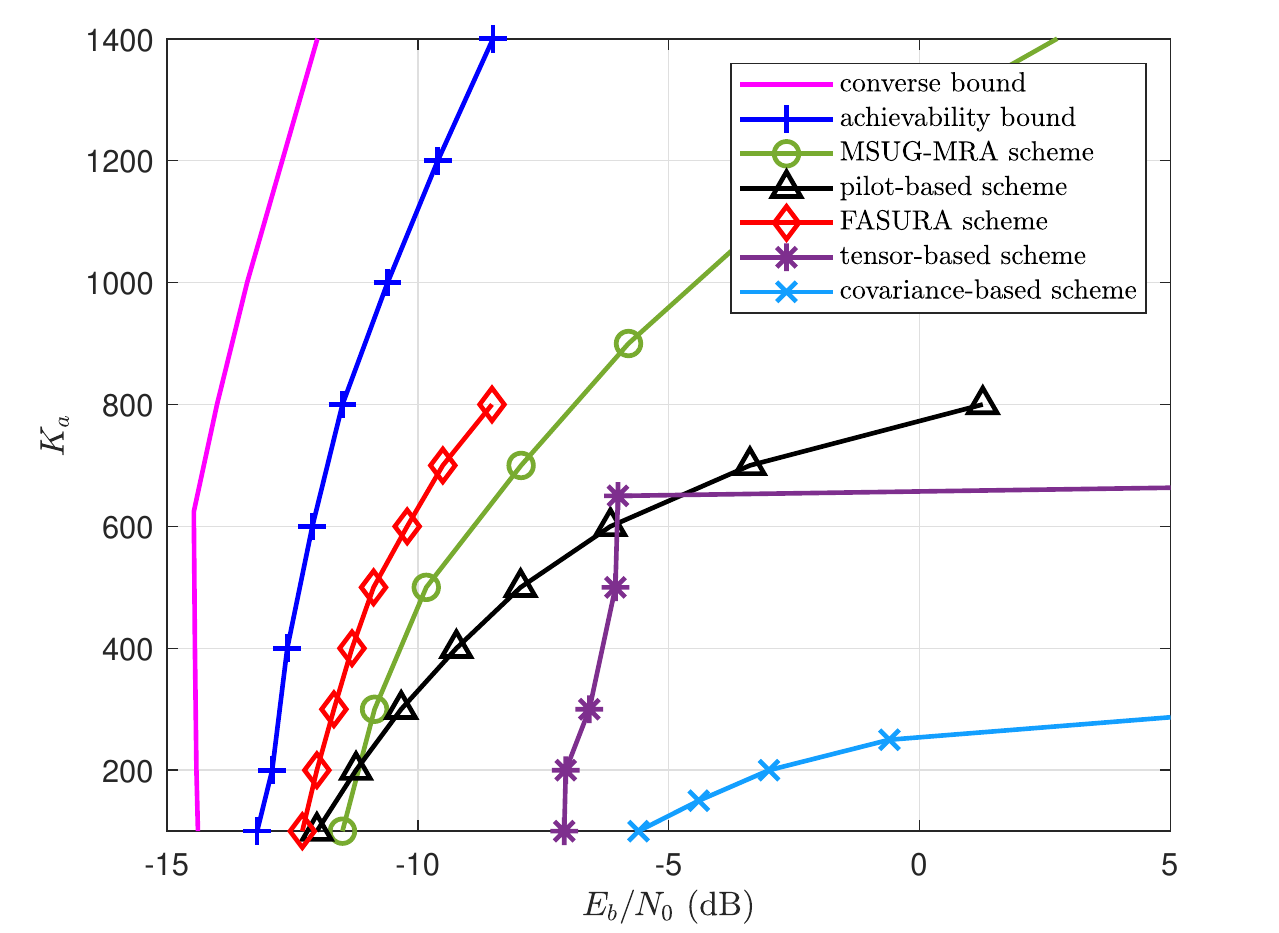
\includegraphics[width=0.85\linewidth]{fig/fig5.png}
\caption{MIMO 준정적 페이딩 채널에서 URA의 기존 기법과 이론적 달성 가능성 한계 및 역 한계의 비교. $K_a$는 고정되어 있고 알려져 있다고 가정하며, $n=3200$, $J=100$비트, $L=50$, $\epsilon_{\mathrm{MD}}=\epsilon_{\mathrm{FA}}=0.025$인 경우이다.}
\end{figure}

\subsubsection{실용 기법과의 비교}

앞에서 세운 유한 부호 길이 한계는 실용 기법을 평가하는 이론적 기준점이 된다. 그림~5에서는 [53]에서 유도한 MIMO 준정적 페이딩 채널의 URA에 대한 유한 부호 길이 달성 가능성 한계와 역 한계(구 위에 균등하게 분포한 부호어 사용)를, [119, 120, 121, 122, 123]에서 제안한 기존 최신 기법과 비교한다. 설정은 부호 길이 $n=3200$, 페이로드 크기 $J=100$비트, 기지국 안테나 수 $L=50$, 목표 미검출 확률과 오경보 확률 $\epsilon_{\mathrm{MD}}=\epsilon_{\mathrm{FA}}=0.025$이다. 최신 기법의 핵심 구현 사항은 다음과 같다. MSUG-MRA 기법은 [120, Fig.~4]와 같이 평가한다. 이 기법은 $n$을 $S$개의 슬롯으로 나누는 슬롯 구조를 쓴다. 각 활성 사용자는 슬롯 하나를 무작위로 고른다. 그 슬롯에서 전송하는 $J$비트 메시지는 $D$개의 직교 파일럿 구간(각 $B_p$비트)과 $J-DB_p$비트의 부호화 구간으로 나뉘며, $G$개의 서로 다른 인터리버-전력 그룹 할당으로 성능을 높인다. 파일럿 기반 기법은 [121, Fig.~7]과 같이 평가한다. 이 기법은 데이터를 각각 16비트와 84비트인 두 부분으로 나눈다. 첫 부분에는 길이 1152의 ``파일럿''을 쓰고, 둘째 부분은 길이 2048의 폴라 부호로 부호화한다. FASURA 기법은 [122, Fig.~4]와 같이 평가하며, 파일럿 기반 기법과 마찬가지로 메시지를 두 부분으로 나눈다. [121]과 다른 점은 길이 $L=9$인 확산 수열을 쓴다는 점, 활성 수열을 검출하는 방법, 그리고 채널/기호 추정 기법이다. 텐서 기반 기법은 [123]과 같이 평가한다. 이 기법은 BCH 외부 부호와 함께 텐서 서명 $(8,5,5,4,4)$를 쓰며, 오류 확률 $\epsilon=0.1$을 허용한다. 공분산 기반 기법은 [119]에서 제안되었다. 이 기법은 16슬롯 프레임을 쓰는데, 각 슬롯은 길이가 200이고, 트리 부호 패리티 프로파일 $[0,7,8,8,9,\dots,9,13,14]$에 따른 15비트를 포함한다. 그림~5에서 보듯 기존 기법은 $K_a$가 작을 때는 경쟁력 있는 에너지 효율을 유지한다. 그러나 $K_a$가 커질수록 성능이 더 많이 떨어지고, 이론적 한계에 비해 더 높은 비트당 에너지 $E_b/N_0$를 요구한다. 따라서 $K_a$가 큰 경우에는 더 진보하고 에너지 효율이 높은 기법 설계가 필요하다.
